\documentclass[final]{beamer}
%% Possible paper sizes: a0, a0b, a1, a2, a3, a4.
%% Possible orientations: portrait, landscape
%% Font sizes can be changed using the scale option.
\usepackage[size=a0,orientation=portrait,scale=1.1]{beamerposter}

\usetheme{gemini}
\usecolortheme{smu}
\useinnertheme{rectangles}

% ====================
% Packages
% ====================

\usepackage[utf8]{inputenc}
\usepackage{graphicx}
\usepackage{booktabs}
\usepackage{tikz}
\usepackage{pgfplots}

% =====================
% Packages added by me
% =====================

\usepackage{chemformula} % para fórmulas químicas
\usepackage[version=4]{mhchem}      % alternativa para ecuaciones químicas
\usepackage[backend=biber,style=numeric, sorting=none, doi=false, url=false]{biblatex}
\usepackage{float}
\usepackage{subcaption}
\usepackage{amsmath}
\usetikzlibrary{shapes.geometric, arrows.meta, positioning}
\usepackage{ragged2e} %Justificar texto en bloques

% ====================
% Lengths
% ====================

% If you have N columns, choose \sepwidth and \colwidth such that
% (N+1)*\sepwidth + N*\colwidth = \paperwidth
\newlength{\sepwidth}
\newlength{\colwidth}
\setlength{\sepwidth}{0.03\paperwidth}
\setlength{\colwidth}{0.45\paperwidth}

\newcommand{\separatorcolumn}{\begin{column}{\sepwidth}\end{column}}

% ====================
% Logo (optional)
% ====================

% LaTeX logo taken from https://commons.wikimedia.org/wiki/File:LaTeX_logo.svg
% use this to include logos on the left and/or right side of the header:
\logoright{ 
\includegraphics[height=8cm]{logos/logo-right.png}}
\logoleft{ \hspace*{2cm} 
\includegraphics[height=8cm]{logos/logo-left.png}}

% ====================
% Footer (optional)
% ====================

\footercontent{
	Facultad de Química. UNAM \hfill
	\insertdate \hfill
	\href{jorgerosas005@gmail.com}{\texttt{jorgerosas005@gmail.com}}
}
% (can be left out to remove footer)

% ====================
% My own customization
% - BibLaTeX
% - Boxes with tcolorbox
% - User-defined commands
% ====================
% ====================
% BibLaTeX
% ====================

%\usepackage[backend=biber,
%	bibstyle=authoryear,
%	citestyle=authoryear,
%	style=numeric,
%	maxcitenames=2,
%	maxbibnames=20, % limit the length of list of names (authors/editors/etc.)
%	sorting=none, % sort references by year (descending), name, title
%	dashed=false, % show authors instead of dash in publications having the same authors
%	giveninits=true % render authors' given name initials and not the full given names
%	oi=false, url=false
%]{biblatex}
%% Biblatex with Beamer bibliography icons
\setbeamertemplate{bibliography item}{%
	\ifboolexpr{ test {\ifentrytype{book}} or test {\ifentrytype{mvbook}}
		or test {\ifentrytype{collection}} or test {\ifentrytype{mvcollection}}
		or test {\ifentrytype{reference}} or test {\ifentrytype{mvreference}} }
	{\setbeamertemplate{bibliography item}[book]}
	{\ifentrytype{online}
		{\setbeamertemplate{bibliography item}[online]}
		{\setbeamertemplate{bibliography item}[article]}}%
	\usebeamertemplate{bibliography item}}
\defbibenvironment{bibliography}
{\list{}
	{\settowidth{\labelwidth}{\usebeamertemplate{bibliography item}}%
		\setlength{\leftmargin}{\labelwidth}%
		\setlength{\labelsep}{\biblabelsep}%
		\addtolength{\leftmargin}{\labelsep}%
		\setlength{\itemsep}{\bibitemsep}%
		\setlength{\parsep}{\bibparsep}}}
{\endlist}
{\item}
%% Redefine \refname
\renewcommand{\bibname}{References}
%% Redefine \parencite to use square brackets instead of braces
\DeclareCiteCommand{\parencite}
{\usebibmacro{prenote}}
{\usebibmacro{citeindex}%
	\printtext[bibhyperref]{[\usebibmacro{cite}]}}
{\multicitedelim}
{\usebibmacro{postnote}}
%% Highlight author names using Beamer data annotation
%% Usage: add a new line `author+an = {<author-order>=highlight}` to an entry
%% For example: author+an = {3=highlight} => highlight the 3rd author name
\AtBeginBibliography{
	\renewcommand*{\mkbibnamegiven}[1]{%
		\ifitemannotation{highlight}
		{\textbf{#1}}
		{#1}%
	}
	
	\renewcommand*{\mkbibnamefamily}[1]{%
		\ifitemannotation{highlight}
		{\textbf{#1}}
		{#1}%
	}
}

% ====================
% Boxes with tcolorbox
% ====================
\usepackage[most]{tcolorbox}

%%% Beamer colors in boxes

\newcommand{\beamercolorsinboxes}[1]{
	\setbeamercolor{itemize item}{fg=#1!75!black}
	\setbeamercolor{itemize/enumerate body}{fg=#1!65!white}
	\setbeamercolor{itemize/enumerate subbody}{fg=#1!65!white}
	\setbeamercolor{item projected}{fg=white, bg=#1!75!black}
}

%%% Highlight Oval Box
\newtcbox{\xmybox}[1][red]{on line,
	arc=7pt,colback=#1!10!white,colframe=#1!50!black,
	before upper={\rule[-3pt]{0pt}{10pt}},boxrule=1pt,
	boxsep=0pt,left=6pt,right=6pt,top=2pt,bottom=2pt}
%%% Box for stating problems
%%%%%%%%
%Usage: (similar for infobox)
%	\begin{defbox}{title}
	%		contents
	%	\end{defbox}
%%%%%%%%
\newtcolorbox{defbox}[1]{%
	enhanced,
	attach boxed title to top 	left={xshift=5mm,yshift=-5mm,yshifttext=-5mm},
	colback=cyan!5!white,
	colframe=cyan!75!black,
	coltitle=cyan!80!black,
%	left=0mm,right=0mm,top=2mm,bottom=0mm,
	title={#1},
	fonttitle=\bfseries\large, fontupper=\color{cyan!65!white},
	boxed title style={colback=cyan!5!white,colframe=cyan!75!black},
	before upper={
		\beamercolorsinboxes{cyan}
	}
}%
%%% Box for announcement
\newtcolorbox{infobox}[1]{%
	enhanced,
	attach boxed title to top 	left={xshift=5mm,yshift=-5mm,yshifttext=-5mm},
	colback=yellow,
	colframe=red!75!black,
	coltitle=red!75!black,
%	left=0mm,right=0mm,top=2mm,bottom=0mm,
	title={#1},
	fonttitle=\bfseries\large, fontupper=\color{red!65!white},
	boxed title style={colback=yellow,colframe=red!75!black},
	before upper={
		\beamercolorsinboxes{red}
	}
}%
%%% Box for example
\newtcolorbox{exabox}[1]{%
	enhanced,
	attach boxed title to top 	left={xshift=5mm,yshift=-5mm,yshifttext=-5mm},
	colframe=brown!75!black,colback=brown!5!white,coltitle=brown!50!brown!75!black,
%	left=0mm,right=0mm,top=2mm,bottom=0mm,
	title={#1},
	fonttitle=\bfseries\large, fontupper=\color{brown!65!white},
	boxed title style={colback=brown!5!white,coltitle=brown!50!brown!75!black},
	before upper={
		\beamercolorsinboxes{brown}
	}
}%
%%% Theorem Box
%%%%%%%%
%Usage: (similar for conjecture, lemma, etc.)
%	\begin{thm}{title}{nameref}
	%		contents
	%	\end{thm}
% Use \ref{thm:nameref} to refer to the theorem
%%%%%%%%
%%%% Use \newtcbtheorem[number within=section]{thm} to number within each section
\newtcbtheorem[]{thm}%
{Theorem}{attach boxed title to top 	left={xshift=5mm,yshift=-5mm,yshifttext=-5mm},
	enhanced jigsaw,
	%	top=2mm,bottom=0mm,left=0mm,right=0mm,
	fonttitle=\bfseries\large,fontupper=\itshape\color{blue!65!white},
	colframe=blue!75!black,colback=blue!5!white,coltitle=blue!50!blue!75!black,
	boxed title style={colback=blue!5!white,coltitle=blue!50!blue!75!black},
	before upper={
		\beamercolorsinboxes{blue}
	}
}{thm}%
%%% Proposition Box
\newtcbtheorem[use counter from=thm]{prop}%
{Proposition}{attach boxed title to top 	left={xshift=5mm,yshift=-5mm,yshifttext=-5mm},
	enhanced jigsaw,
	%	top=2mm,bottom=0mm,left=0mm,right=0mm,
	fonttitle=\bfseries\large,fontupper=\itshape,
	colframe=gray!75!black,colback=gray!5!white,coltitle=gray!50!gray!75!black,
	boxed title style={colback=gray!5!white,coltitle=gray!50!gray!75!black},
	before upper={
		\beamercolorsinboxes{gray}
	}
}{prop}%
%%% Conjecture Box
\newtcbtheorem[use counter from=thm]{conj}%
{Conjecture}{attach boxed title to top 	left={xshift=5mm,yshift=-5mm,yshifttext=-5mm},
	enhanced jigsaw,
	%	top=2mm,bottom=0mm,left=0mm,right=0mm,
	fonttitle=\bfseries\large,fontupper=\slshape,
	colframe=orange!75!black,colback=orange!5!white,coltitle=orange!50!orange!75!black,
	boxed title style={colback=orange!5!white,coltitle=orange!50!orange!75!black},
	before upper={
		\beamercolorsinboxes{orange}
	}
}{conj}%
%%% Lemma Box
\newtcbtheorem[use counter from=thm]{lem}%
{Lemma}{attach boxed title to top 	left={xshift=5mm,yshift=-5mm,yshifttext=-5mm},
	enhanced jigsaw,
	%	top=2mm,bottom=0mm,left=0mm,right=0mm,
	fonttitle=\bfseries\large,fontupper=\itshape,
	colframe=green!75!black,colback=green!5!white,coltitle=green!50!green!75!black,
	boxed title style={colback=green!5!white,coltitle=green!50!green!75!black},
	before upper={
		\beamercolorsinboxes{green}
	}
}{lem}%
%%% Claim Box
\newtcbtheorem[use counter from=thm]{clm}%
{Claim}{attach boxed title to top 	left={xshift=5mm,yshift=-5mm,yshifttext=-5mm},
	enhanced jigsaw,
	%	top=2mm,bottom=0mm,left=0mm,right=0mm,
	fonttitle=\bfseries\large,fontupper=\itshape,
	colframe=pink!75!black,colback=pink!5!white,coltitle=pink!50!pink!75!black,
	boxed title style={colback=pink!5!white,coltitle=pink!50!pink!75!black},
	before upper={
		\beamercolorsinboxes{pink}
	}
}{clm}%

%% Reference Sources
\addbibresource{referencias.bib}
\renewcommand{\pgfuseimage}[1]{\includegraphics[scale=2.0]{#1}}

\title{Estudio de la solvatación del ion \ce{Cu^{2+}} en medios polares mediante dinámica molecular con DFT/M06-2X}

\author{Jorge Angel Rosas Martínez \inst{1} \and César Iván León Pimentel \inst{2}}
\institute[shortinst]{\inst{1} Facultad de Química, UNAM }

\date{Agosto 2025}

\begin{document}
	
\begin{frame}[t]
	
	\begin{columns}[t]
		\separatorcolumn

		\begin{column}{\colwidth}
			\begin{block}{I N T R O D U C C I Ó N}

				\justifying

				La solvatación del ion cobre (II) \ce{Cu^{2+}} es fundamental para una vasta gama de procesos químicos y biológicos, desde su papel crítico en las actividades enzimáticas, el transporte de oxígeno y la transferencia de electrones \cite{Wa-2023-01, Wa-2024-03} hasta su implicación en trastornos neurodegenerativos \cite{Cu-2014-02}. Una característica central que gobierna su química en fase de solución es la distorsión de Jahn-Teller, consecuencia directa de su configuración electrónica $d^9$ \cite{Cu-2019-01}, la cual imparte una considerable labilidad estructural y una dinámica compleja a su primera capa de solvatación.\\ Este fenómeno ha sido estudiado extensamente en disolución acuosa, generando un vasto cuerpo de conocimiento, aunque no exento de debate sobre la estructura y dinámica de su primera esfera de coordinación. Existe un consenso emergente que apunta a una coexistencia dinámica de especies con números de coordinación 5 y 6 \cite{Wa-2023-01}. Sin embargo, la información disponible para la solvatación de este ion en metanol es considerablemente más escasa y, en ocasiones, contradictoria, con estudios experimentales que reportan números de coordinación promedio que varían desde 4 hasta 6 \cite{Me-2025-01}. \\ Para abordar esta ambigüedad en la información de la literatura se realizó un estudio de Dinámica Molecular Ab initio (AIMD por sus siglas en inglés) basada en la Teoría de los Funcionales de la Densidad (DFT por sus siglas en inglés) utilizando M06-2X. Analizamos los complejos de coordinación \ce{[Cu(H2O)_{40}]^{2+}} y \ce{[Cu(CH3OH)_{40}]^{2+}} con objeto de contrastar nuestros resultados obtenidos con el resto de trabajos similares con agua y presentar por primera vez en la literatura un estudio riguroso de esta naturaleza para caracterizar la solvatación del \ce{Cu^{2+}} en metanol.


			\end{block}

		\end{column}

		\separatorcolumn

		\begin{column}{\colwidth}

			\begin{alertblock}{C L U S T E R S}

				\begin{figure}[H]
					\centering
					% Fila superior: Complejos con Metanol
					\begin{subfigure}[b]{0.27\textwidth}
						\centering
						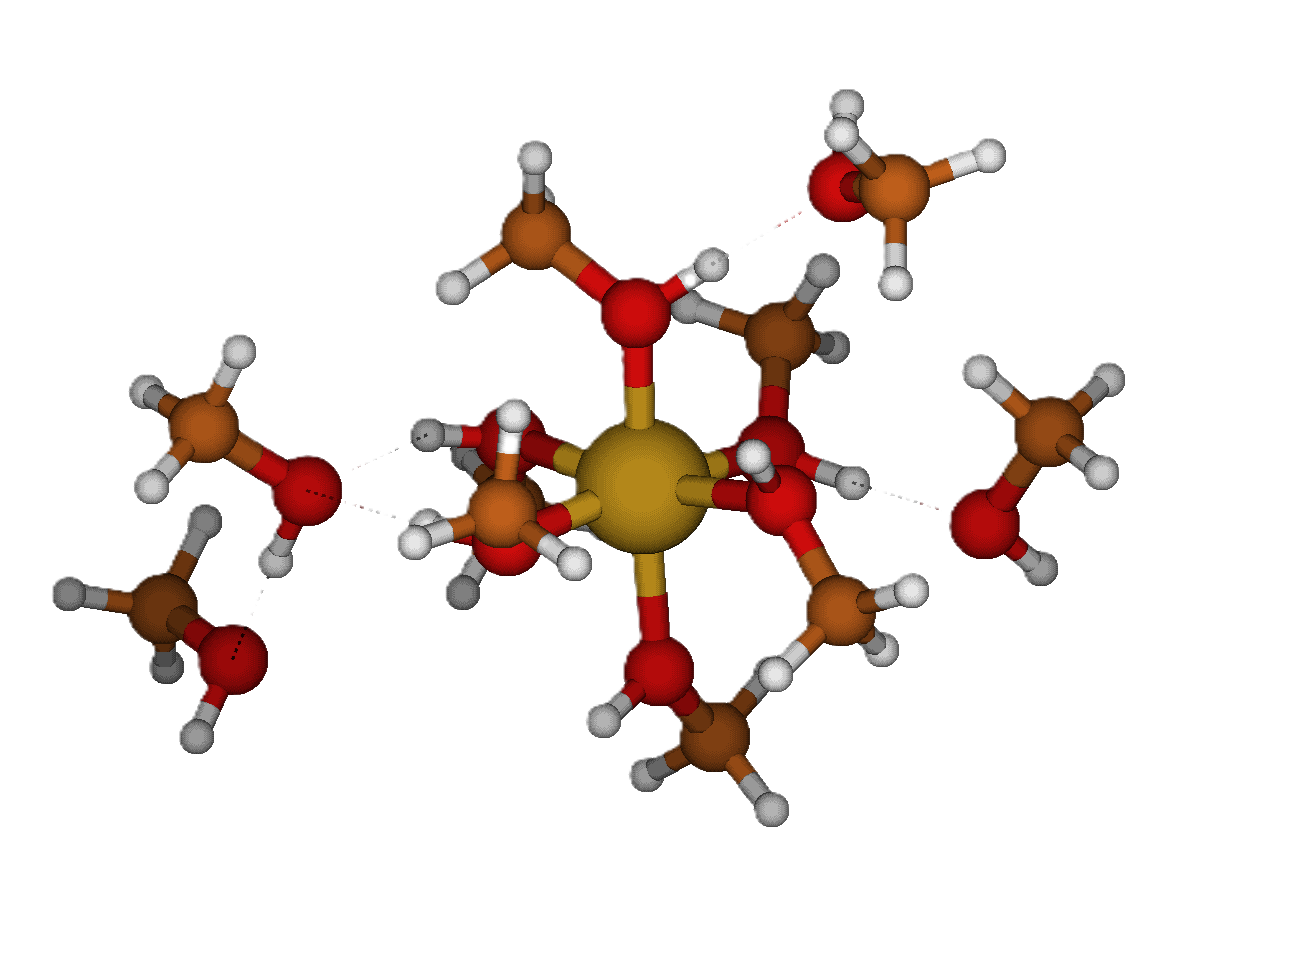
\includegraphics[width=\textwidth]{logos/Cu-10CH4O.png}
						\caption{\ce{[Cu(CH3OH)_{10}]^{2+}}}
						\label{fig:cu-10ch4o}
					\end{subfigure}%
					\hfill
					\begin{subfigure}[b]{0.27\textwidth}
						\centering
						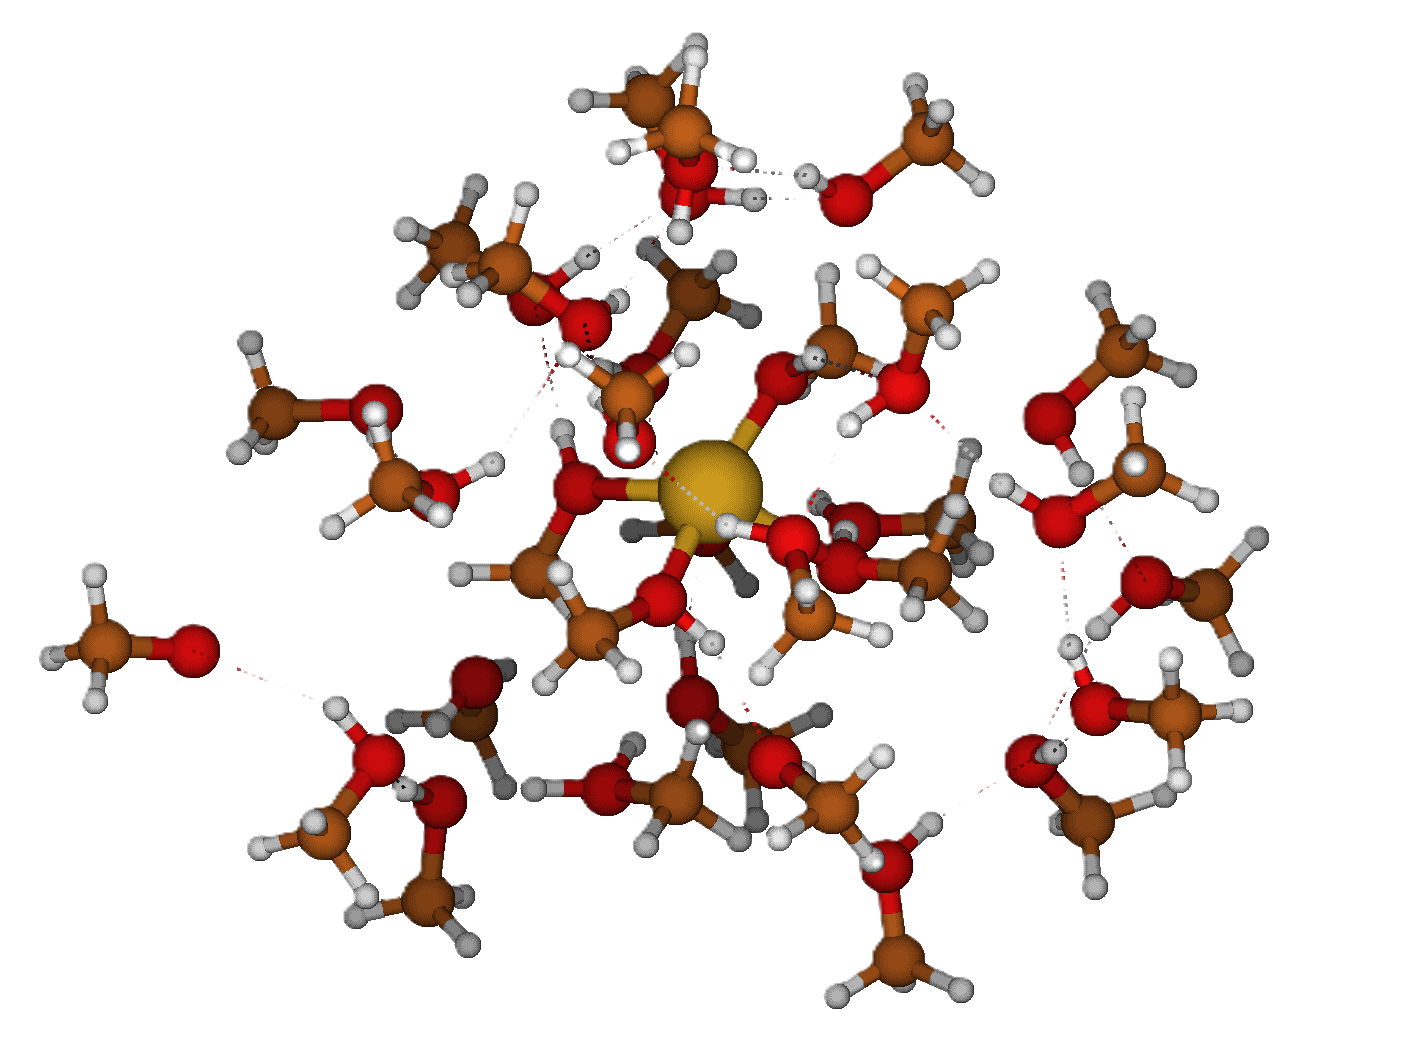
\includegraphics[width=\textwidth]{logos/Cu-30CH4O.png}
						\caption{\ce{[Cu(CH3OH)_{30}]^{2+}}}
						\label{fig:cu-30ch4o}
					\end{subfigure}%
					\hfill
					\begin{subfigure}[b]{0.27\textwidth}
						\centering
						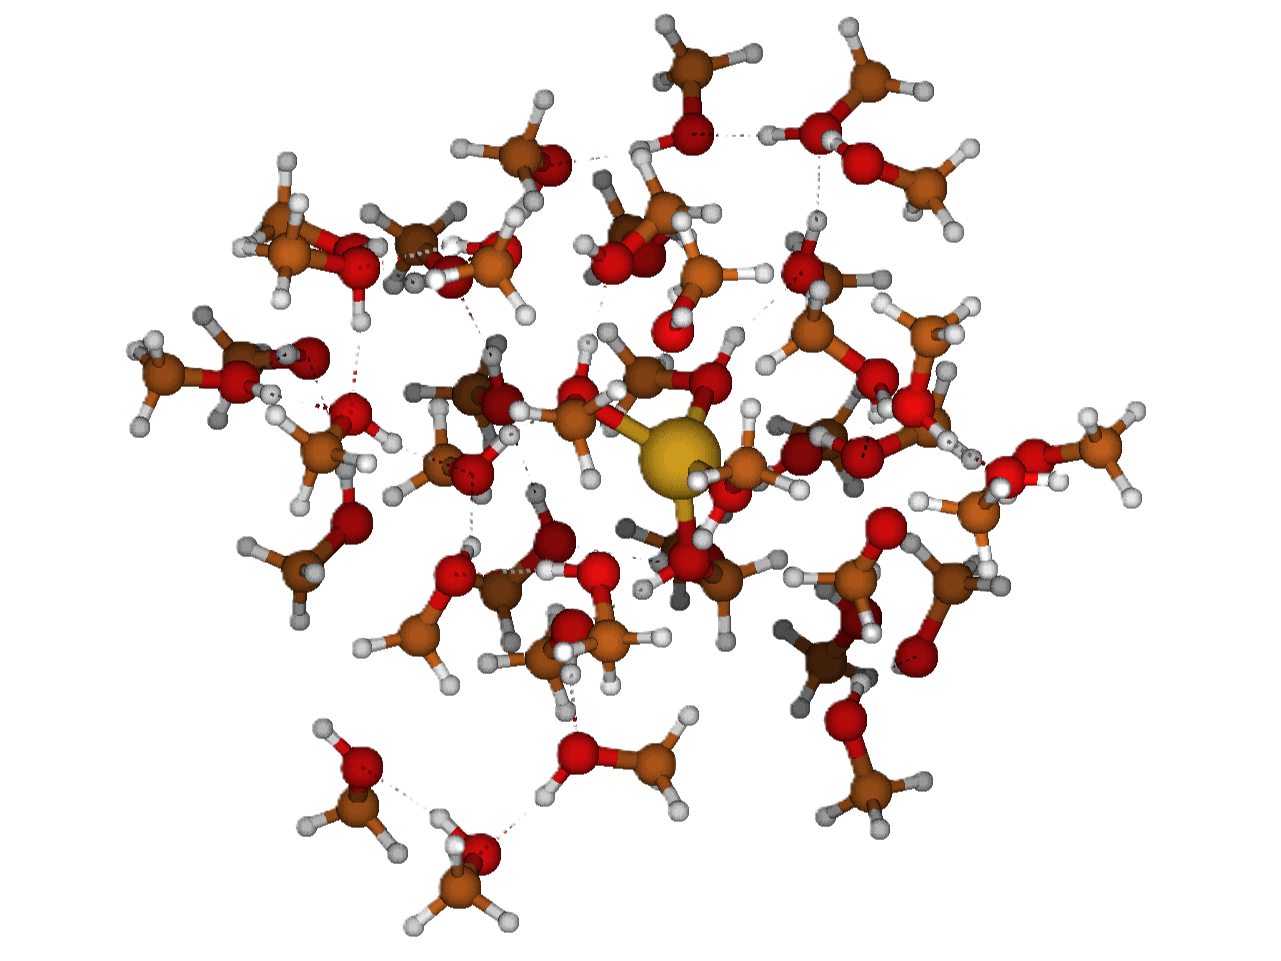
\includegraphics[width=\textwidth]{logos/Cu-40CH4O.png}
						\caption{\ce{[Cu(CH3OH)_{40}]^{2+}}}
						\label{fig:cu-40ch4o}
					\end{subfigure}
					
					\vspace{1em} % Espacio vertical entre las filas de imágenes
					
					% Fila inferior: Complejos con Agua
					\begin{subfigure}[b]{0.27\textwidth}
						\centering
						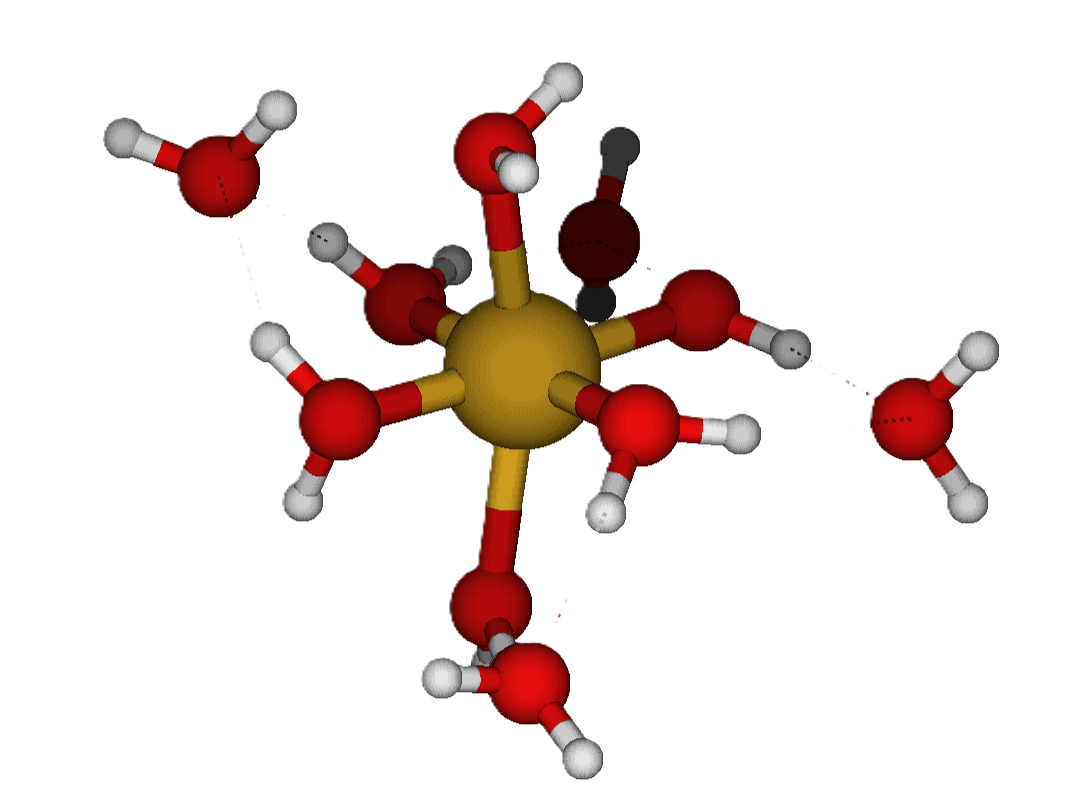
\includegraphics[width=\textwidth]{logos/Cu-10H2O.png}
						\caption{\ce{[Cu(H2O)_{10}]^{2+}}}
						\label{fig:cu-10h2o}
					\end{subfigure}%
					\hfill
					\begin{subfigure}[b]{0.27\textwidth}
						\centering
						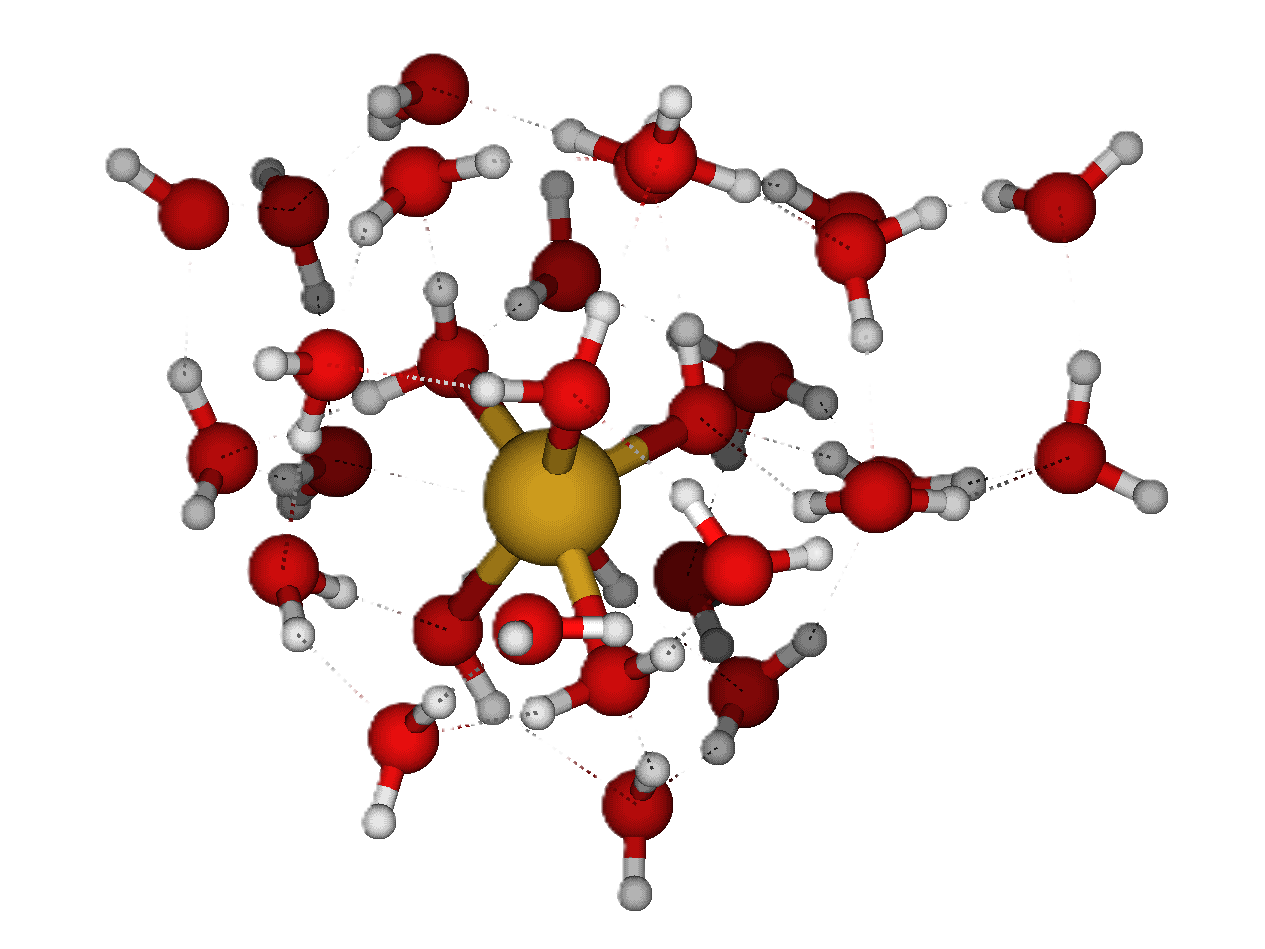
\includegraphics[width=\textwidth]{logos/Cu-30H2O.png}
						\caption{\ce{[Cu(H2O)_{30}]^{2+}}}
						\label{fig:cu-30h2o}
					\end{subfigure}%
					\hfill
					\begin{subfigure}[b]{0.27\textwidth}
						\centering
						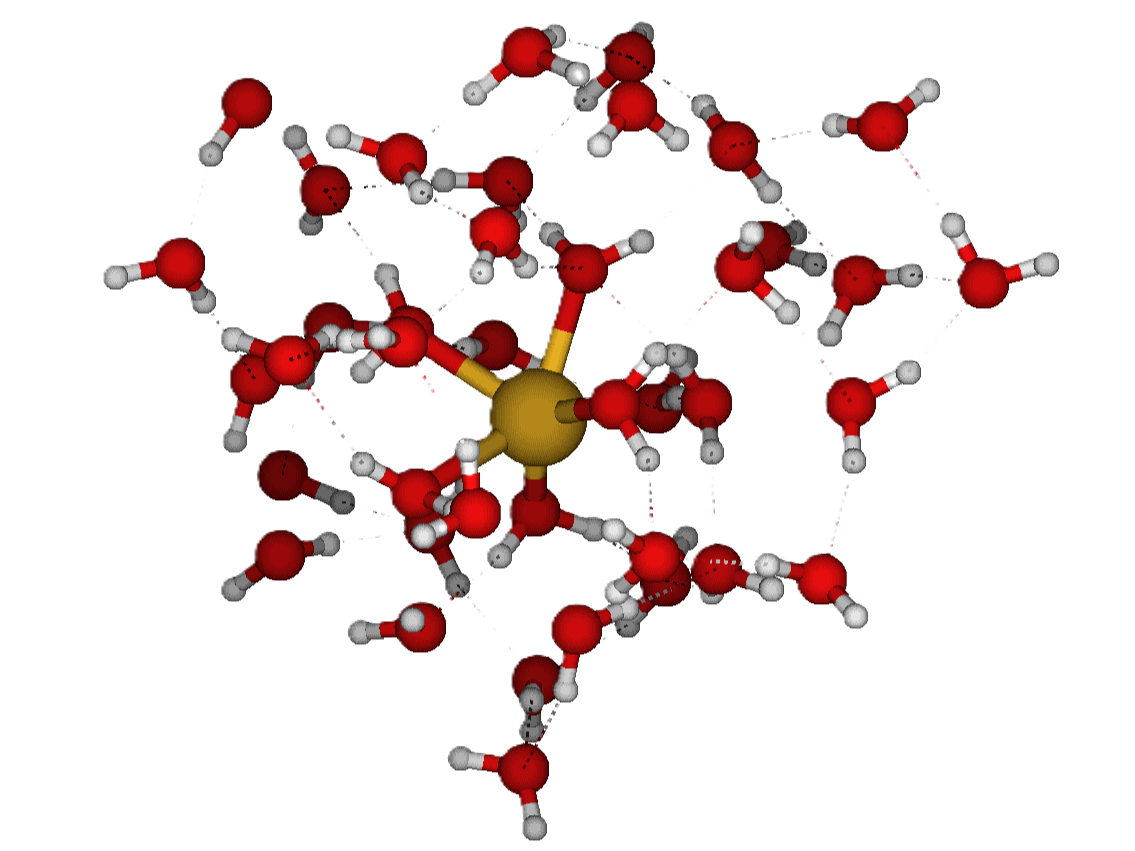
\includegraphics[width=\textwidth]{logos/Cu-40H2O.png}
						\caption{\ce{[Cu(H2O)_{40}]^{2+}}}
						\label{fig:cu-40h2o}
					\end{subfigure}
					
					\caption{Estructuras de solvatación óptimas para los sistemas \ce{[Cu(CH3OH)_{n}]^{2+}} (fila superior) y \ce{[Cu(H2O)_{n}]^{2+}} (fila inferior), con $n = 10,\ 30,\ 40$.}
					\label{fig:estructuras_solvatacion}
				\end{figure}				

			\end{alertblock}

		\end{column}
		
		\separatorcolumn
	
	\end{columns}

	\begin{columns}[t]
	
		\begin{column}{2\colwidth+\sepwidth}
			\begin{exampleblock}{M E T O D O L O G Í A}{}
				
				\begin{figure}[H]
					\centering
					\begin{tikzpicture}[font=\footnotesize\sffamily,
						node distance = 8mm and 15mm, % Distancia vertical y horizontal
						block/.style = {rectangle, draw, text centered, rounded corners,
										minimum height=2.2cm, align=center},
						diamond_dec/.style = {diamond, draw, text centered, aspect=2,
											inner sep=1pt, text width=2.5cm},
						line/.style = {-{Stealth[length=2.5mm]}}
						]

						% --- Fila Superior ---
						\node[block] (cond) {\textbf{Inicialización}  \\ $R^{N}(t=0)$};
						\node[block, right=of cond] (opt_structure) {\textbf{Optimizar estructura} \\ {\text{Minimizar energía}} \\ $R^{N}_{min}(0)$};
						\node[block, right=of opt_structure](init_vel) {\textbf{Velocidades} \\ \textbf{iniciales} \\$V^{N}(t=0)$};
						\node[block, right=of init_vel] (t_step) { \textbf{Bucle SCF} \\ $t^{(n)}$};



						% --- Fila Intermedia (Bucle SCF) ---
						\node[block, right=3cm of t_step] (propose_rho){ \textbf{Proponer} \\$\rho^{(n)}(r)$};
						\node[block, below=2.3cm of propose_rho] (build_h) {\textbf{Construir hamiltoniano} \\ $H^{(n)}_{KS} = -\frac{1}{2} \nabla^2 + V_{\text{ext}} + V_H^{(n)} + V_{xc}^{(n)}$};
						\node[block, right=of build_h] (solve_ks) {\textbf{Resolver ecuaciones} \\ \textbf{de Kohn-Sham} \\ $H^{(n)}_{KS} \psi_i = \epsilon_i\psi_i$};
						\node[block, right=of solve_ks] (calc_rho) {\textbf{Calcular nueva densidad} \\ $\rho^{(n+1)}(r) = \sum_{i=1}^{N_{occ}} |\psi_i(r)|^2$};
						\node[diamond_dec, above=1.8cm of calc_rho, xshift=0cm] (scf_check) {  \textbf{¿Converge?}  };
						\node[block, right=of scf_check, xshift=1cm] (forces) {\textbf{Calcular energía y fuerzas} \\ $E[\rho] = T_s[\rho] + V_H[\rho] + E_{xc}[\rho] + V_{ext}[\rho]$ \\ $F_I = -\nabla_{R_I} E[\rho]$};

						% --- Fila Inferior (Bucle de Dinámica) ---
						% ***** LÍNEA MODIFICADA AQUÍ *****
						\node[block, below=5.5cm of forces] (vel_update) {\textbf{Actualizar velocidades} \\ \text{Yoshida 7 + Nosé-Hoover} \\  $V^{N}(t + \Delta t)$ , $T \approx 300\,\text{K}$ };
						\node[block, left=11.5cm of vel_update] (pos_update) {\textbf{Actualizar posiciones} \\ \text{Yoshida 7} \\ $R^{N}( t + \Delta t)$};

						% --- Inicio y Fin ---
						\node[block, left=of cond] (start) {Inicio};
						\node[diamond_dec, left=11.5cm of pos_update] (main_loop_check) {¿$t < 22.5\,\text{ps}$?};
						\node[block, left=of main_loop_check] (analysis) {\textbf{Análisis}};
						\node[block, left=of analysis] (end) {Fin};

						% --- Conexiones con Flechas ---
						% Flujo principal
						\draw[line] (start) -- (cond);
						\draw[line] (cond) -- (opt_structure);
						\draw[line] (opt_structure) -- (init_vel);
						\draw[line] (init_vel) -- (t_step);
						\draw[line] (t_step) -- (propose_rho);

						% Bucle SCF
						\draw[line] (propose_rho) -- (build_h);
						\draw[line] (build_h) -- (solve_ks);
						\draw[line] (solve_ks) -- (calc_rho);
						\draw[line] (calc_rho) -- (scf_check);
						\draw[line] (scf_check) -- node[above] {Sí} (forces);
						\draw[line] (scf_check.west) -- ++(-0.5,0) -| node[below, pos=0.25] {$\rho^{(n)}(r) = \rho^{(n+1)}(r)$}  node[above, pos=0.25] {No} (propose_rho.east);

						% Bucle de Dinámica
						\draw[line] (forces) -- (vel_update);
						\draw[line] (vel_update) -- (pos_update);
						\draw[line] (pos_update) -- (main_loop_check);

						% Bucle principal y final
						\draw[line] (main_loop_check.north) -| node[left, pos=0.8] {Si} (t_step.south);
						\draw[line] (main_loop_check) -- node[below, pos=0.5] {No} (analysis);
						\draw[line] (analysis) -- (end);

						

					\end{tikzpicture}
					\caption{Diagrama general de cálculo.}
					\label{fig:metodologia}
				\end{figure}

				Para la fase de inicialización de $R^{N}(t=0)$ se utilizó Packmol v2, se hicieron una serie de optimizaciones para estructuras desde$n = 1,\ 2,\ \ldots,\ 10,\ 30,\ 40$ para agua y metanol (ver figura 3) y determinar la elección de base 6-31G*. Los parámetros de la simulación fueron los siguientes:

				\begin{itemize}
					\item Funcional intercambio y correlación M06-2X con 6-31G*
					\item Las velocidades iniciales se calculan conforme a la distribución de Maxwell-Boltzmann a $T \approx 300\,\text{K}$
					\item La duración de la DM fue 22.5 ps con $\Delta t = 0.5\,\text{fm}$ (45,000 ciclos de cálculo)
					\item Ensamble NVT con termostato Nosé-Hoover en cadena (4) $T \approx 300\,\text{K}$ e integrador de orden superior Yoshida 7
				\end{itemize}

				Los cálculos de optimización y las dinámicas moleculares se realizaron en Orca v6.1 \cite{orca}.

			\end{exampleblock}		

		\end{column}

	\end{columns}

	\begin{columns}[t]

		\separatorcolumn
		
		\begin{column}{\colwidth}
			
			\begin{block}{E N E R G Í A}{}

				%%%
				\begin{figure}[H]
					\centering
					\begin{minipage}[b]{0.48\textwidth}
						\centering
						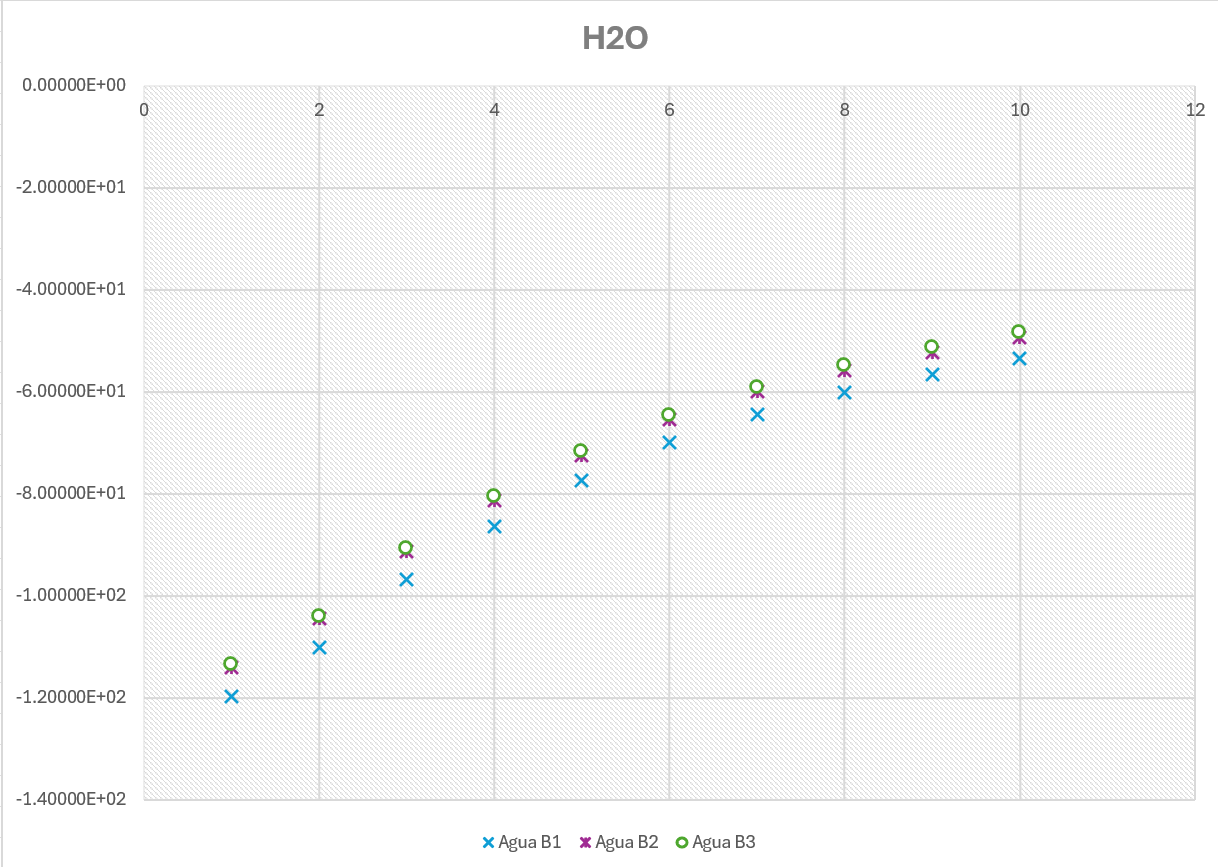
\includegraphics[width=\textwidth]{logos/bases_agua.png}
					\end{minipage}%
					\hfill
					\begin{minipage}[b]{0.48\textwidth}
						\centering
						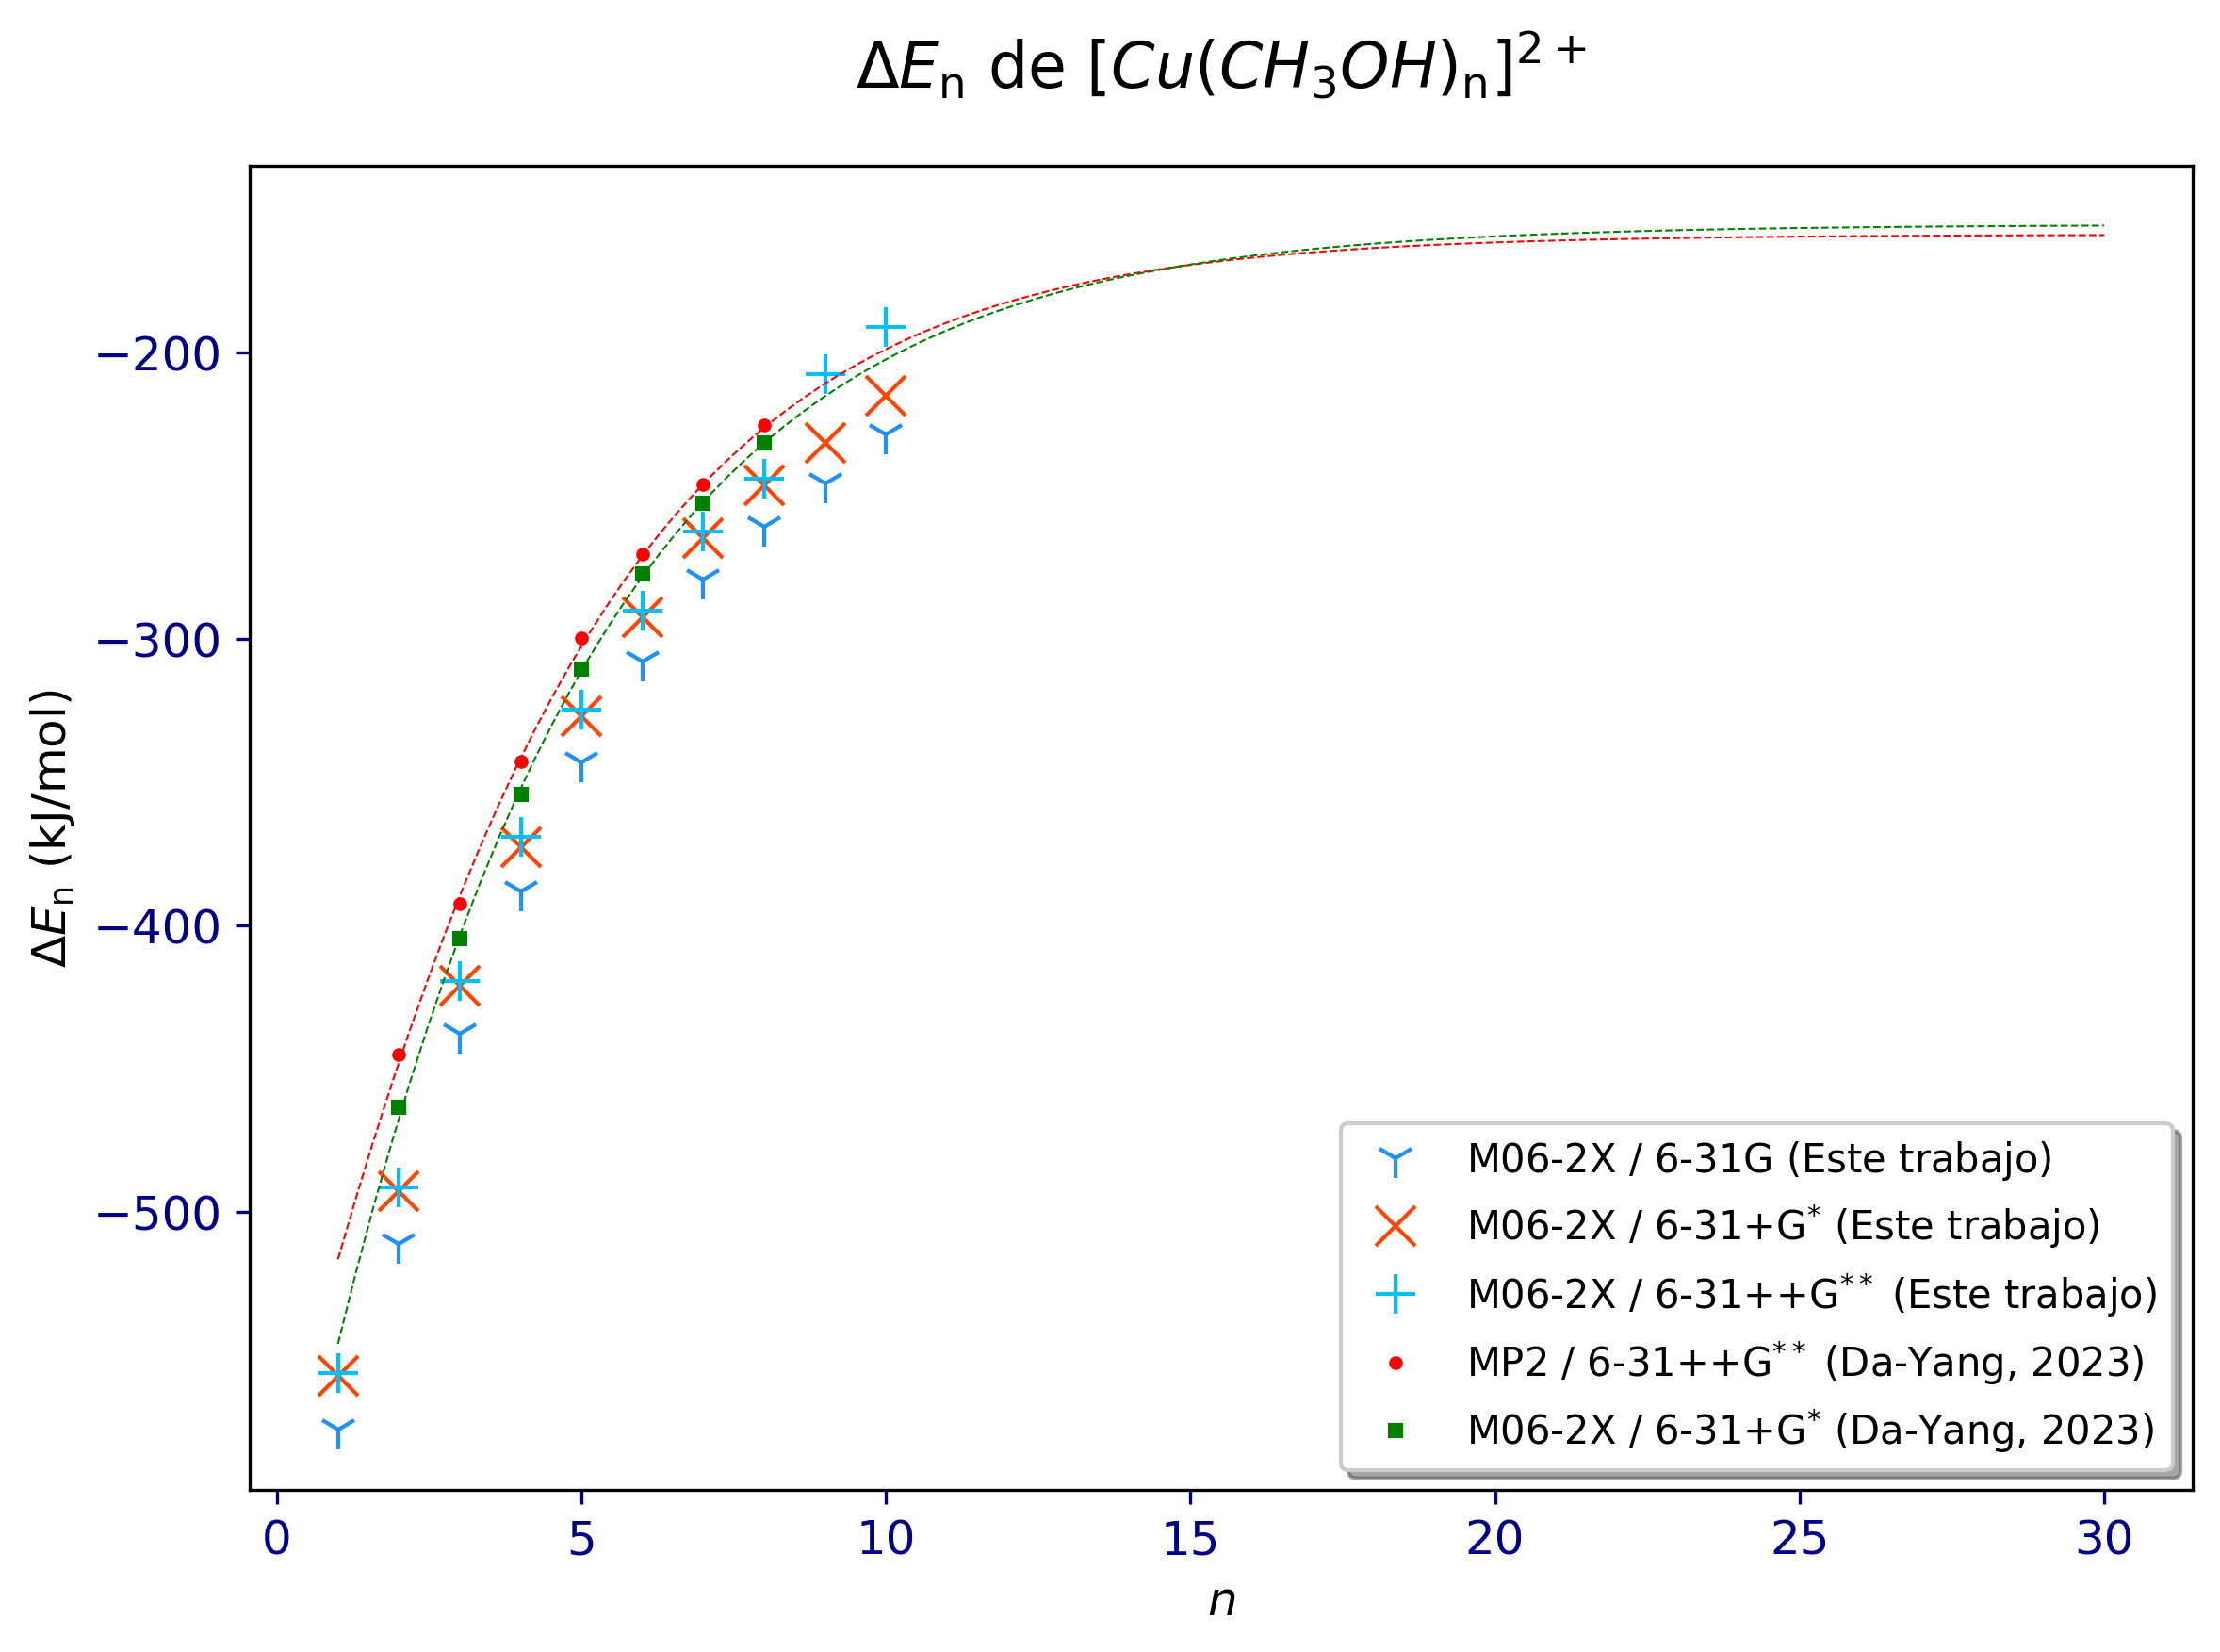
\includegraphics[width=\textwidth]{logos/bases_metanol.png}
					\end{minipage}

					\caption{Energías de enlace por molécula de solvente calculada para las estructuras de solvatación óptimas de \ce{[Cu(H2O)_{n}]^{2+}} (izquierda) y \ce{[Cu(CH3OH)_{n}]^{2+}} (derecha), con $n = 1,\ 2,\ \ldots,\ 10,\ 30,\ 40$, mediante cálculos de optimización con los niveles de teoría 6-31G$^\ast$, 6-31+G$^\ast$ y 6-31++G$^{\ast\ast}$. Resultados obtenidos con MP2 \cite{Me-2022-01} y validación de M06-2X respecto a MP2 \cite{Me-2023-01}.}
					\label{fig:bases}
				\end{figure}
				
			\end{block}
			
			\begin{exampleblock}{C O N C L U S I O N E S}{}
				Conclusiones preeliminares:
				. \\
				. \\
				. \\
				. \\
				. \\
				. \\
				. \\
				. \\
				. \\
				. \\
				. \\
				. \\
				. \\
				. \\
				. \\
				. \\			
				. \\
				. \\


			\end{exampleblock}		

		\end{column}
	
		\separatorcolumn
		
		\begin{column}{\colwidth}
		
			\begin{block}{C A R A C T E R I Z A C I Ó N }{}
				
				\begin{figure}[H]
					\centering
					% Primera imagen
					\begin{minipage}[c]{0.49\textwidth} % Adjust width as needed, ensure total < 1.0\textwidth
						\centering
						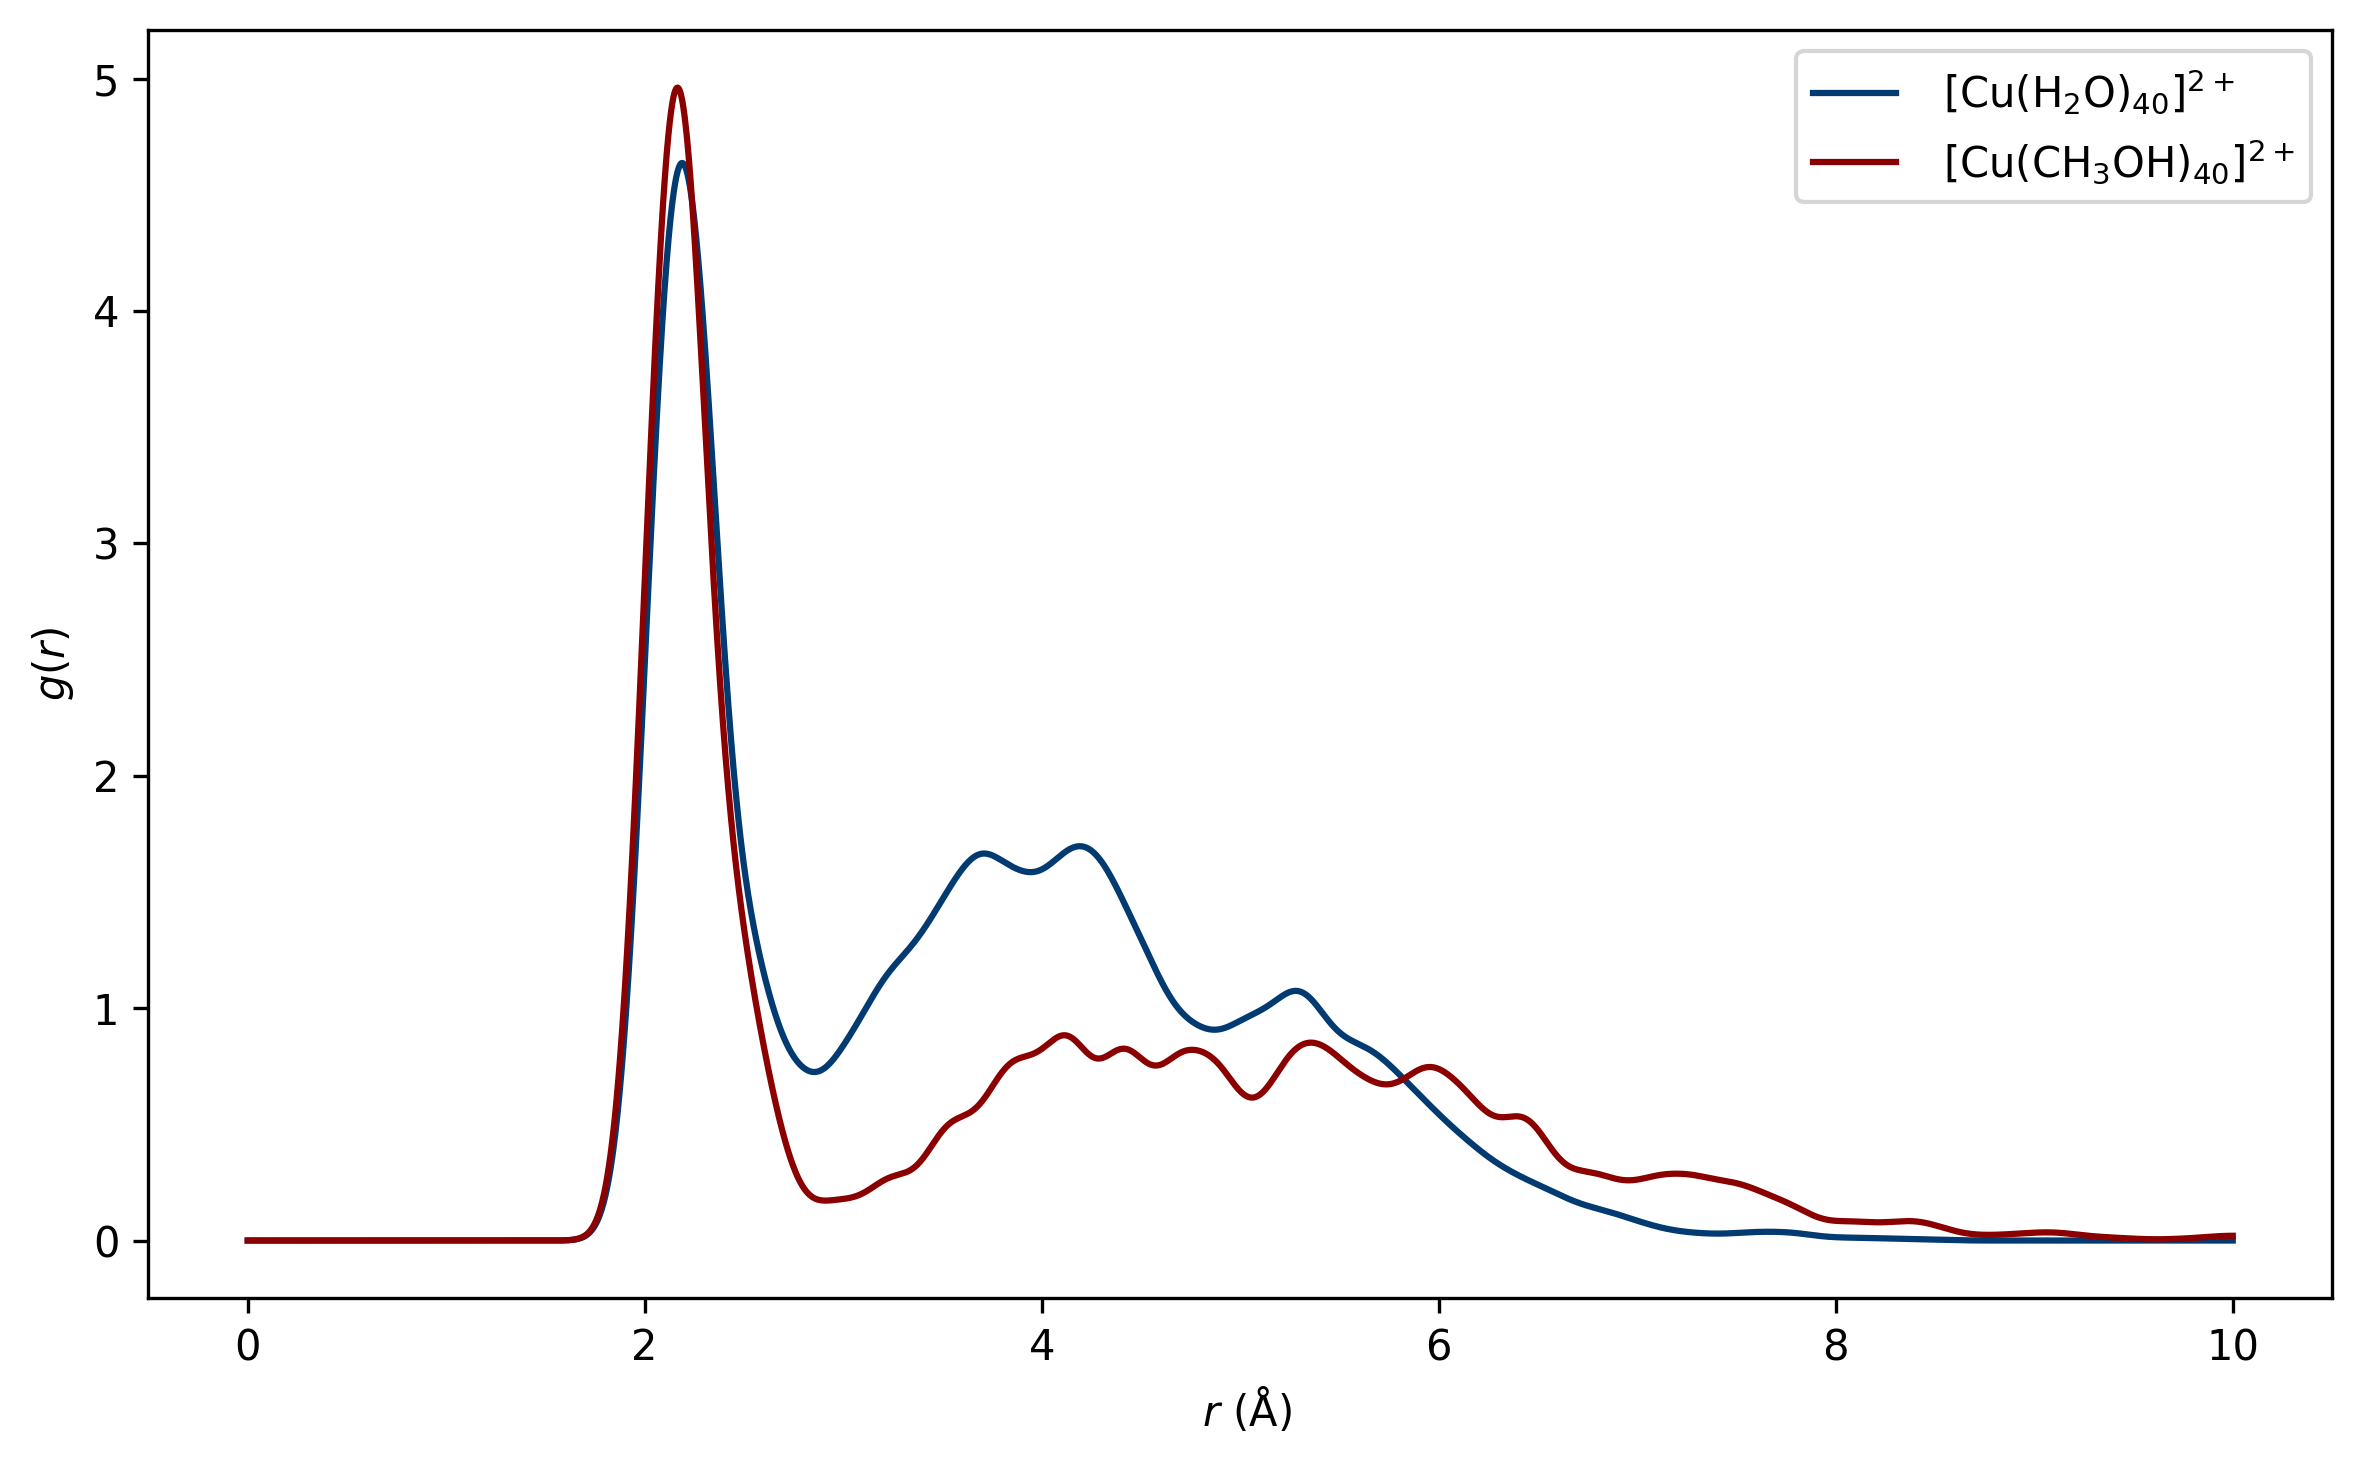
\includegraphics[width=\textwidth]{logos/RDF-OUTPUT-HISTOGRAMA.png}
						\caption{Función de distribución radial para el ion \ce{Cu^{2+}} en metanol (\ce{CH_{4}O}) y agua (\ce{H_{2}O}).}
						\label{fig:rdfcu40ch4o}
					\end{minipage}% <--- Important: No space here!
					\hfill % Adds flexible space between minipages, or remove if you want them tight
					% Segunda imagen
					\begin{minipage}[c]{0.49\textwidth} % Adjust width as needed
						\centering
						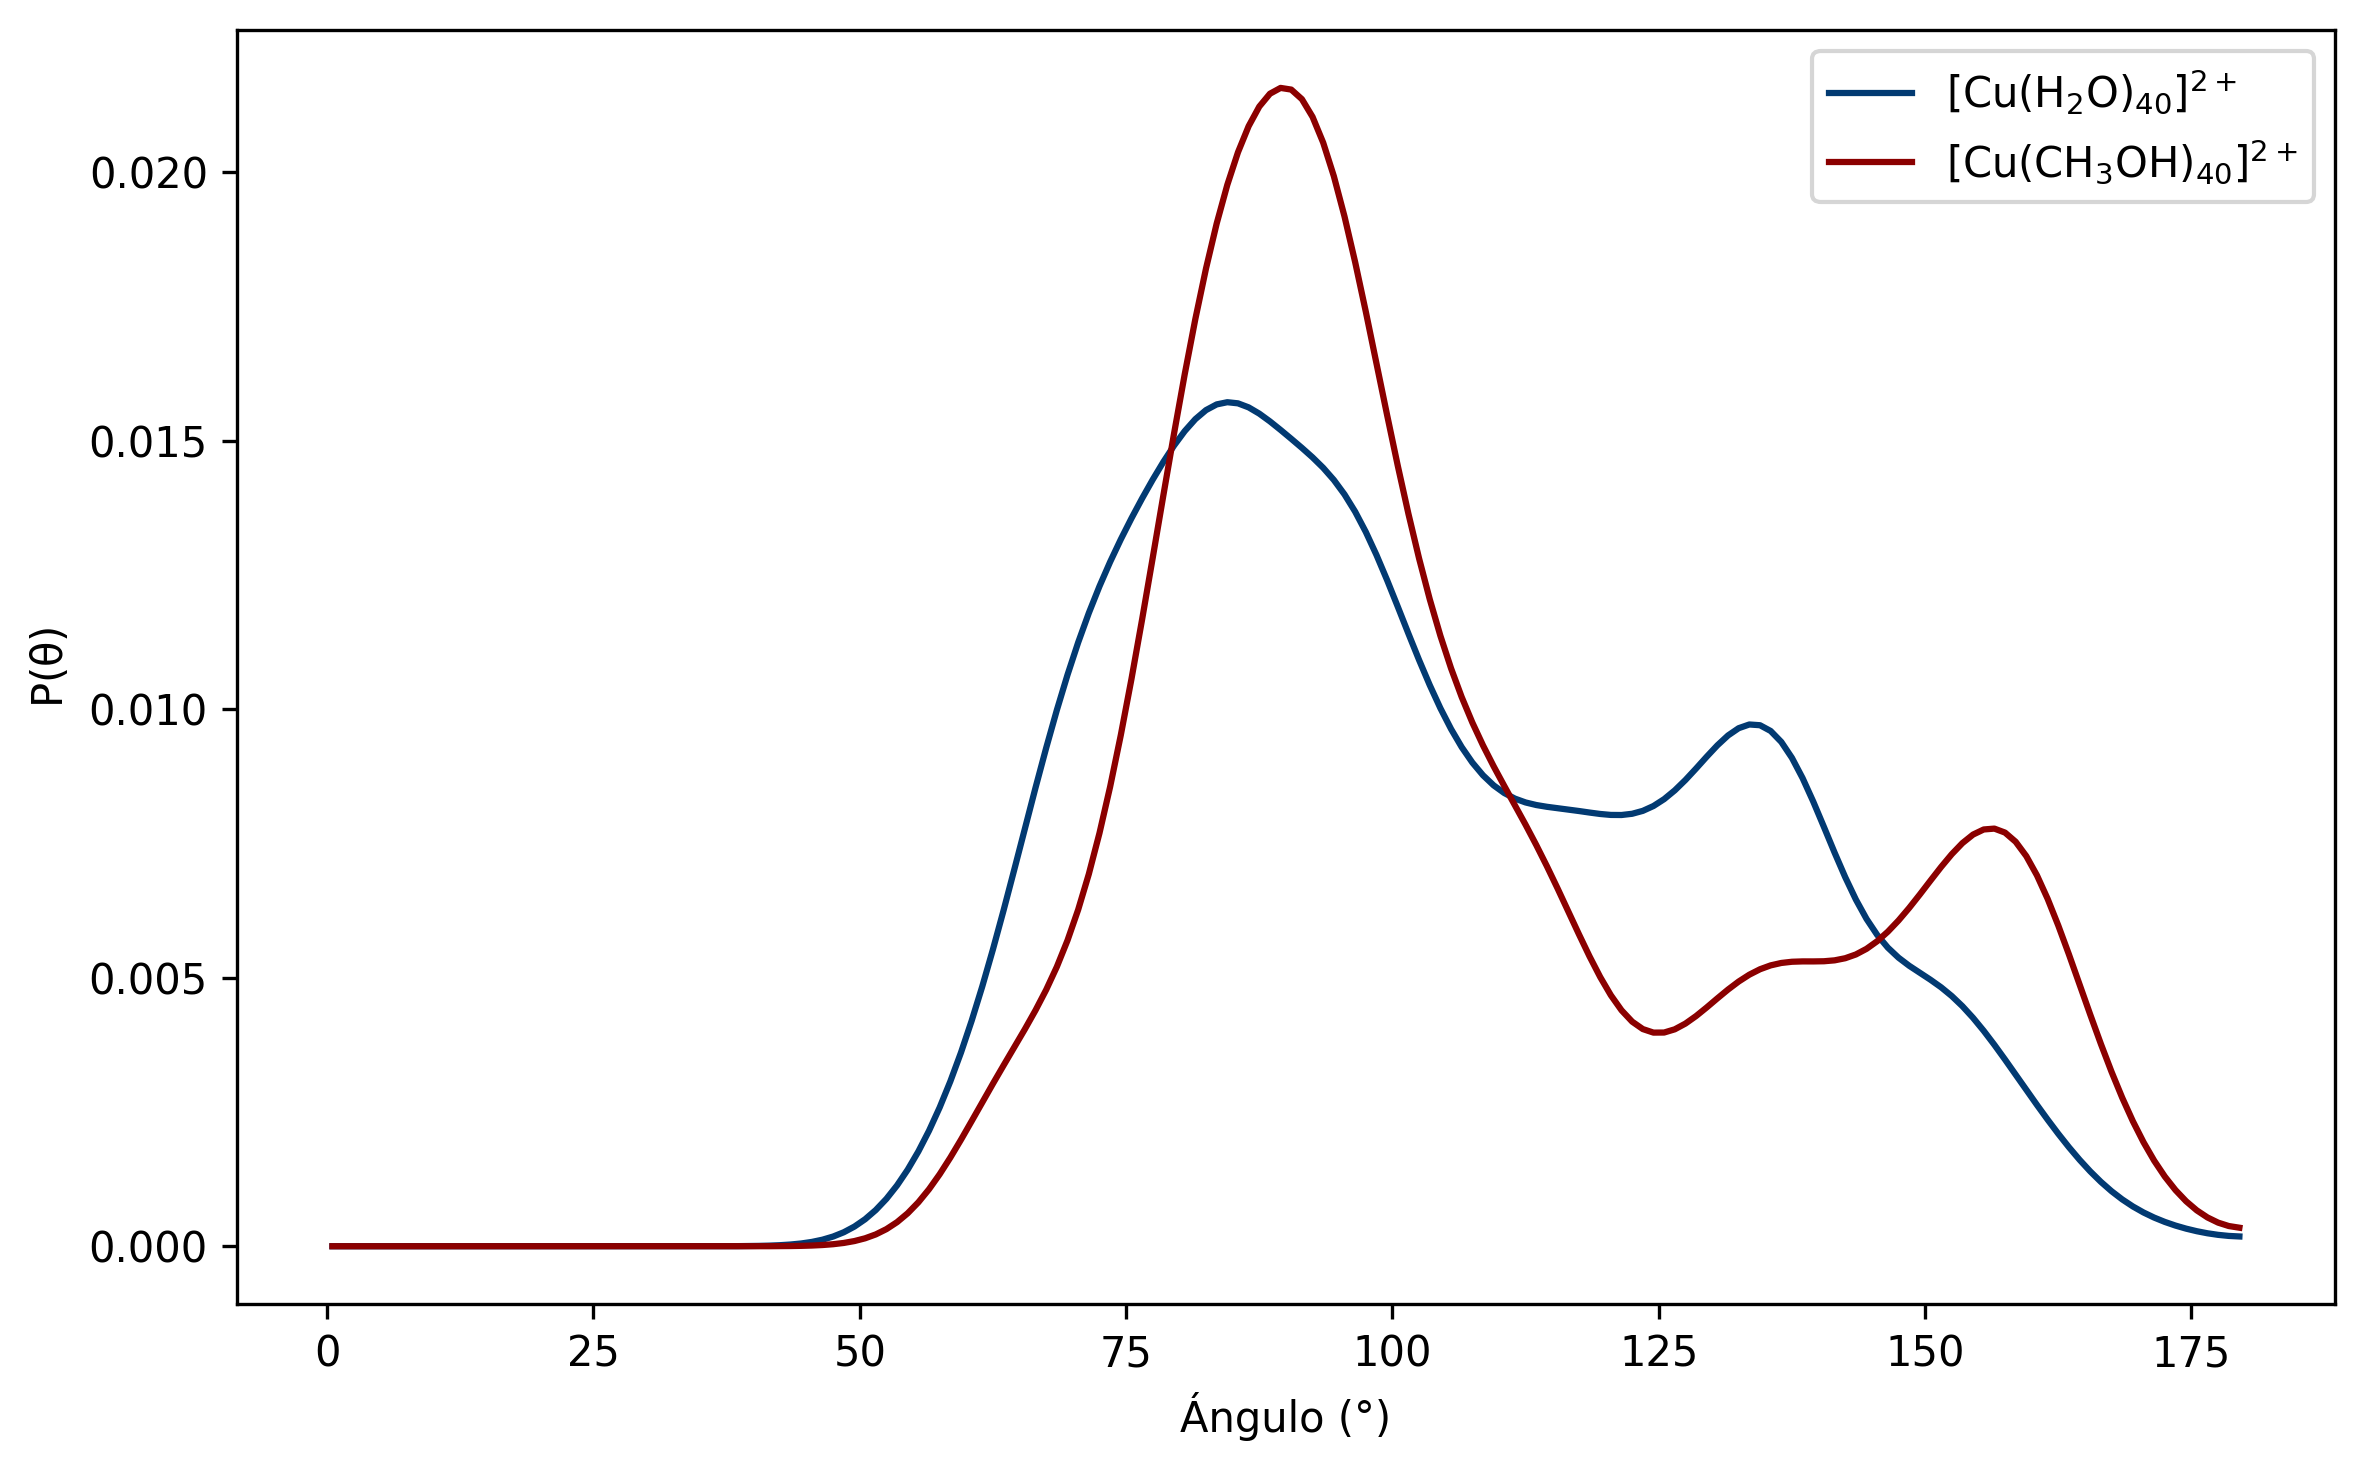
\includegraphics[width=\textwidth]{logos/ADF-OUTPUT-HISTOGRAMA.png}
						\caption{Función de distribución angular con $r = 2.9$ para el ion \ce{Cu^{2+}} en metanol (\ce{CH_{4}O}) y agua (\ce{H_{2}O}).}
						\label{fig:adfcu40ch4o}
					\end{minipage}
				\end{figure}

			\end{block}	

			\begin{block}{References}
				\printbibliography[heading=none]
			\end{block}
		\end{column}
		
		\separatorcolumn
	\end{columns}
\end{frame}
\end{document}